\documentclass[10pt,a4paper]{article}
\usepackage[a4paper, left=3cm, right=3cm, top=3cm, bottom=3cm, headsep=10mm, footskip=12mm]{geometry}
\usepackage[T1]{fontenc}
\usepackage[ngerman, english]{babel}    % mehrsprachiger Textsatz
% babel: letzte Sprache in Optionen zeigt die Sprache des Dokumentes
% und kann durch den Befehl \selectlanguage{} geaendert werden
% Passen Sie die Optionen des babel-Paketes nach Bedarf an!
\usepackage{float}
\usepackage{graphicx}
\usepackage{url}
\usepackage{pdflscape}
\usepackage{mathtools}
\usepackage{amssymb, amsmath, amstext}
\usepackage{amsthm}
\usepackage{xcolor}
\usepackage{nameref}
\usepackage{siunitx}
\usepackage{makecell}
\usepackage{hyperref}
\usepackage{enumitem}
\usepackage[superscript,biblabel]{cite}
\usepackage{caption}
\usepackage{subcaption}
\usepackage{tabularx} 			% Tabellen erzeugen
\usepackage{multirow}			 % Zeilen in Tabellenbearbeitung
\usepackage{multicol} 			% Spalten in Tabellenbearbeitung 
\usepackage{lmodern}                        % Ersatz fuer Computer Modern-Schriften 
\usepackage{amsmath}                                           % zum besseren Aussehen am Bildschirm
\usepackage{booktabs} % für schönere Tabellen
\usepackage{sidecap}
\usepackage{rotating} % für die Landscape-Umgebung
\usepackage{afterpage}
\definecolor{Bluetitle}{HTML}{1F3864}
\definecolor{softbluetitle}{HTML}{274D7E}
\definecolor{Greyish}{HTML}{5A5A5A}
\renewcommand{\refname}{Reference}
\usepackage{array,multirow}
\newcommand{\specialcell}[2][c]{%
	\begin{tabular}[#1]{@{}c@{}}#2\end{tabular}}




\begin{document}
	
	\begin{titlepage}
		\begin{center}
			\begin{figure}[h!tbp]
				
\includegraphics[width=\linewidth]{HUlogo.PNG}
			\end{figure}
			\vspace*{2 cm}
			
			\textcolor{Bluetitle}{\textbf{\huge Charakterisierung
					der Photosynthesepigmente der Nicotina tabacum Pflanze}}\par
			\vspace*{0.5cm}
			\textcolor{softbluetitle}{\textbf{\Large Wildtyp vs FC1-Antisense-Mutante}}\par
			
			\vspace*{2cm}
			
			\textcolor{Greyish}{\textbf{Versuchsdurchführende}}\par
			\textcolor{Greyish}{...}\par

			\vspace*{0.5cm}
			\textcolor{Greyish}{\textbf{Versuchsort}}\par
			\textcolor{Greyish}{..}\par
			\textcolor{Greyish}{..}\par
			\vspace*{0.5cm}
			\textcolor{Greyish}{\textbf{Versuchsbetreuer}}\par
			\textcolor{Greyish}{..}\par
			
			\vspace*{2 cm}
			
			\textcolor{Greyish}{11. Juni 2024}\par
			

			
			
		\end{center}
	\end{titlepage}
		
		\tableofcontents
		

	
	\newpage
	\section{Einführung}
	Photosynthese ist ein biochemischer Prozess der von grünen Pflanzen, einigen Algenarten und bestimmten Bakterien, genutzt wird um Licht zu absorbieren und energetisch nutzbar zu machen. In den höheren Pflanzen sind hierfür die Pigmente Chlorophyll a und b(abgekürzt: Chl a und Chl b), sowie  einige Carotinoide zuständig, welche in Verbindung mit den Pigment-bindenden-Proteinen der Photosysteme I und II, in den Thylakoidmembranen der Chloroplasten zu finden sind. Die Pigmente dienen der aufnahme von Lichtenergie und der Weiterleitung dieser zu den Reaktionszentren, wo eine Elektronentransportkette eingeleitet wird, um als Teil der lichtabhängigen Reaktion, ATP und NADPH zu synthetisieren und letztendlich, während der Dunkelreaktion Glukose zu bilden.\\
	\\
	In diesen Versuch werden die Photosynthesepigmente Chlorophylle und Carotinoide in den Wildtyp und FC1-antisense-Mutant (abgekürzt: Mutant) von der Pflanze Nicotina tabacum untersucht.\\
	Die Ziele der Versuche sieht wie folgt aus:
	
	\begin{itemize}
		\item Charakterisierung der einzelnen Photosynthesepigmente in Wildtyp- und Mutantenpflanze mittels Absorptionsspektrum und Trennung der Pigmentbestandteile mittels Dünnschichtchromatographie (abgekürzt: DC)
		\item  Fluoreszenzeigenschaft von Chlorophylle in wässrigen und organischen Lösemittel und der Einfluss des Mediums auf die Struktur
		\item Stabilitätsuntersuchung von Chlorophylle
	\end{itemize}
	
	
	\section{Material und Methode}
	Die Verdünnungen und Homogenisieren wurde jeweils auf Eis durchgeführt.
		\subsection{Herstellung des Pigmentextraktes}
		Es wurde 0.9965g Pflanzenmaterial des Wildtypens und 0.9960g des Mutantes eingewogen (zwei Blätter der Mutantenpflanze haben weißliche Flecken).\\
		Die Proben wurden mit kalten basischen Aceton (100$\%$ Aceton und 20mM NH$_4$OH) homogenisiert und über einem Miraclothfilter in einem 50mL Falconröhrchen filtriert. Ein Spatelspitze Quarzsand wurde hier als zusätzlichen Zerkleinerungshilfe verwendet.\\
		Flüssiger Extrakt der jeweiligen Pflanzentypen wurde in einem 15mL Falcon vereinigt.
		
		\subsection{Photometrische Bestimmung Chlorophylle a und b}
		Um eine quantitative Bestimmung von  Chlorophyll a und b durchzuführen, wurden zuerst 0.2ml  des Wildtyp-Extrakts (WT) und des der Mutante (MU) in ein 1,5ml Reaktionsgefäß überführt. Anschließend wurde ein Verhälltnis von 1:5 geschaffen, indem 0.8ml basisches Aceton hinzugegeben wurde.  \\
		Das Gemisch wurde gevortext und für eine Minute bei 15.000 rpm herunterzentrifugiert.
		Die photometrische Bestimmung von 1 mL Probevolumen erfolgte bei 470nm, 646nm, 663nm und 720nm wobei 720nm Wellenlänge als Maß für Verunreinigung diente und 470nm als nicht relevanter Kontrollwert.\\
		Als Blank-Lösung wurde das Extraktionslösung (basisches Aceton) verwendet.
		
		\subsection{DC-Trennung Chlorophylle und Carotinoide}\label{text: DC}
		5 mL des basischen Pigmentextraktes vom Wildtyp und Mutant wurde mit 1 mL Petrolether versetzt und 3 mal vorsichtig invertiert.
		Die Proben wurden für 10 Minuten im Eis inkubiert und die obere dunkelgrüne Phase für die weiteren Versuchen in einem 1.5mL Eppendorf Tube überführt.\\
		\\
		50$\mu$L von den Wildtyp- und Mutantenextraktes wurden auf einer Dünnschichtchromatographie-Platte (abgekürzt: DC-Platte) als breites Band aufgetragen.
		In einem mit Laufmittel (Petrolether/Aceton/Isopropanol/Wasser, 400:80:48:1)-abgesättigte DC-Kammer wird die DC-Platte inkubiert und der Lauf wurde gestoppt, als diese 5 mm Abstand zur DC-Plattenkante erreicht hatte.\\
		Die nebeneinanderliegenden Banden vom Wildtyp und Mutant wurde gemeinsam extrahiert (1. und 4. Bande mit Ethanol gelöst und 2. und 3. Bande mit basischen Aceton), bei 15000rpm abzentrifugiert und das Absorptionsspektrum des Überstandes bei $\lambda$ = 350 - 720 nm gemessen. Als Blanklösung diente hier bei den Ethanolproben Ethanol und bei den Acetonproben basisches Aceton.
		\subsection{Fluoreszenz des Chlorophyllextractes}
		Es wurde 0.5mL von den Wildtyp- und Mutantpetroletherextract von Abschnitt \ref{text: DC} und 0.5mL von den Wildtypextraktes in wässrigen Lösung in einem Eppi überführt und am UV-Tisch das Fluoreszenzverhalten beobachtet.
		
		\subsection{Phäophytinbildung}
		
		200 $\mu$L des Petrolextraktes wurde 1:2 mit Aceton verdünnt und dann tropfenweise mit 1M Salzsäure solange zugegeben bis die Farbe von grün zu braun umschlägt.
	
	\section{Ergebnis}
		\subsection{Konzentrationsbestimmung von Chlorophylle im Rohextrakt}
		Die Konzentration von Chlorophyll a und b wurde mit der Gl. \ref{eq:chl a gleichung} und \ref*{eq:chl b gleichung} photometrisch bestimmt.\\
		Es wurde eine Konzentration für Chl a von 2.221$\mu$g/g Frischgewicht und Chl b  von 0.510 $\mu$g/g Frischgewicht für das Wildtyp gemessen. Für die Mutante betrug die Konzentration an Chl a 3.363$\mu$g/g Frischgewicht und Chl b 0.742$\mu$g/g Frischgewicht gemessen.\\
		Rechenweg kann im Anhang (Figure  \ref{fig:Konzentrationsbestimmungrechenweg}) nachvollzogen werden.\\
		\\
		\begin{equation}\label{eq:chl a gleichung}
			\frac{\frac{(12.21 \cdot (A_{663} - A_{720}) - 2.81 \cdot (A_{646} - A_{720}))}{V(Extrakt)} \cdot Verdünnungsfaktor}{m(Frischgewicht)}
		\end{equation}
		\\
		\begin{equation}\label{eq:chl b gleichung}
			\frac{\frac{(20.21 \cdot (A_{663} - A_{720}) - 4.91 \cdot (A_{646} - A_{720}))}{V(Extrakt)} \cdot Verdünnungsfaktor}{m(Frischgewicht)}
		\end{equation}
		
			\begin{table}[H]
				\centering
				\caption{Chlorophyll a und b Konzentration des Rohextraktes vom Wildtyp und Mutant der Nicotina tabacum Pflanze.}
				\label{tab:konzentration chl a und b}
				\begin{tabular}{ccc}
					\toprule
					Typ&c[Chl a] in $\mu$g/g Frischgewicht & c[Chl b] in $\mu$g/g Frischgewicht\\
					\midrule
					Wildtyp& 2.221 & 0.510\\
					Mutant & 3.363 & 0.742\\
					\bottomrule
				\end{tabular}
			\end{table}	
		
		\subsection{Quantitative Bestimmung der Pigmentebestandteile des Rohextraktes}
			
			\begin{figure}[H]
				\centering
				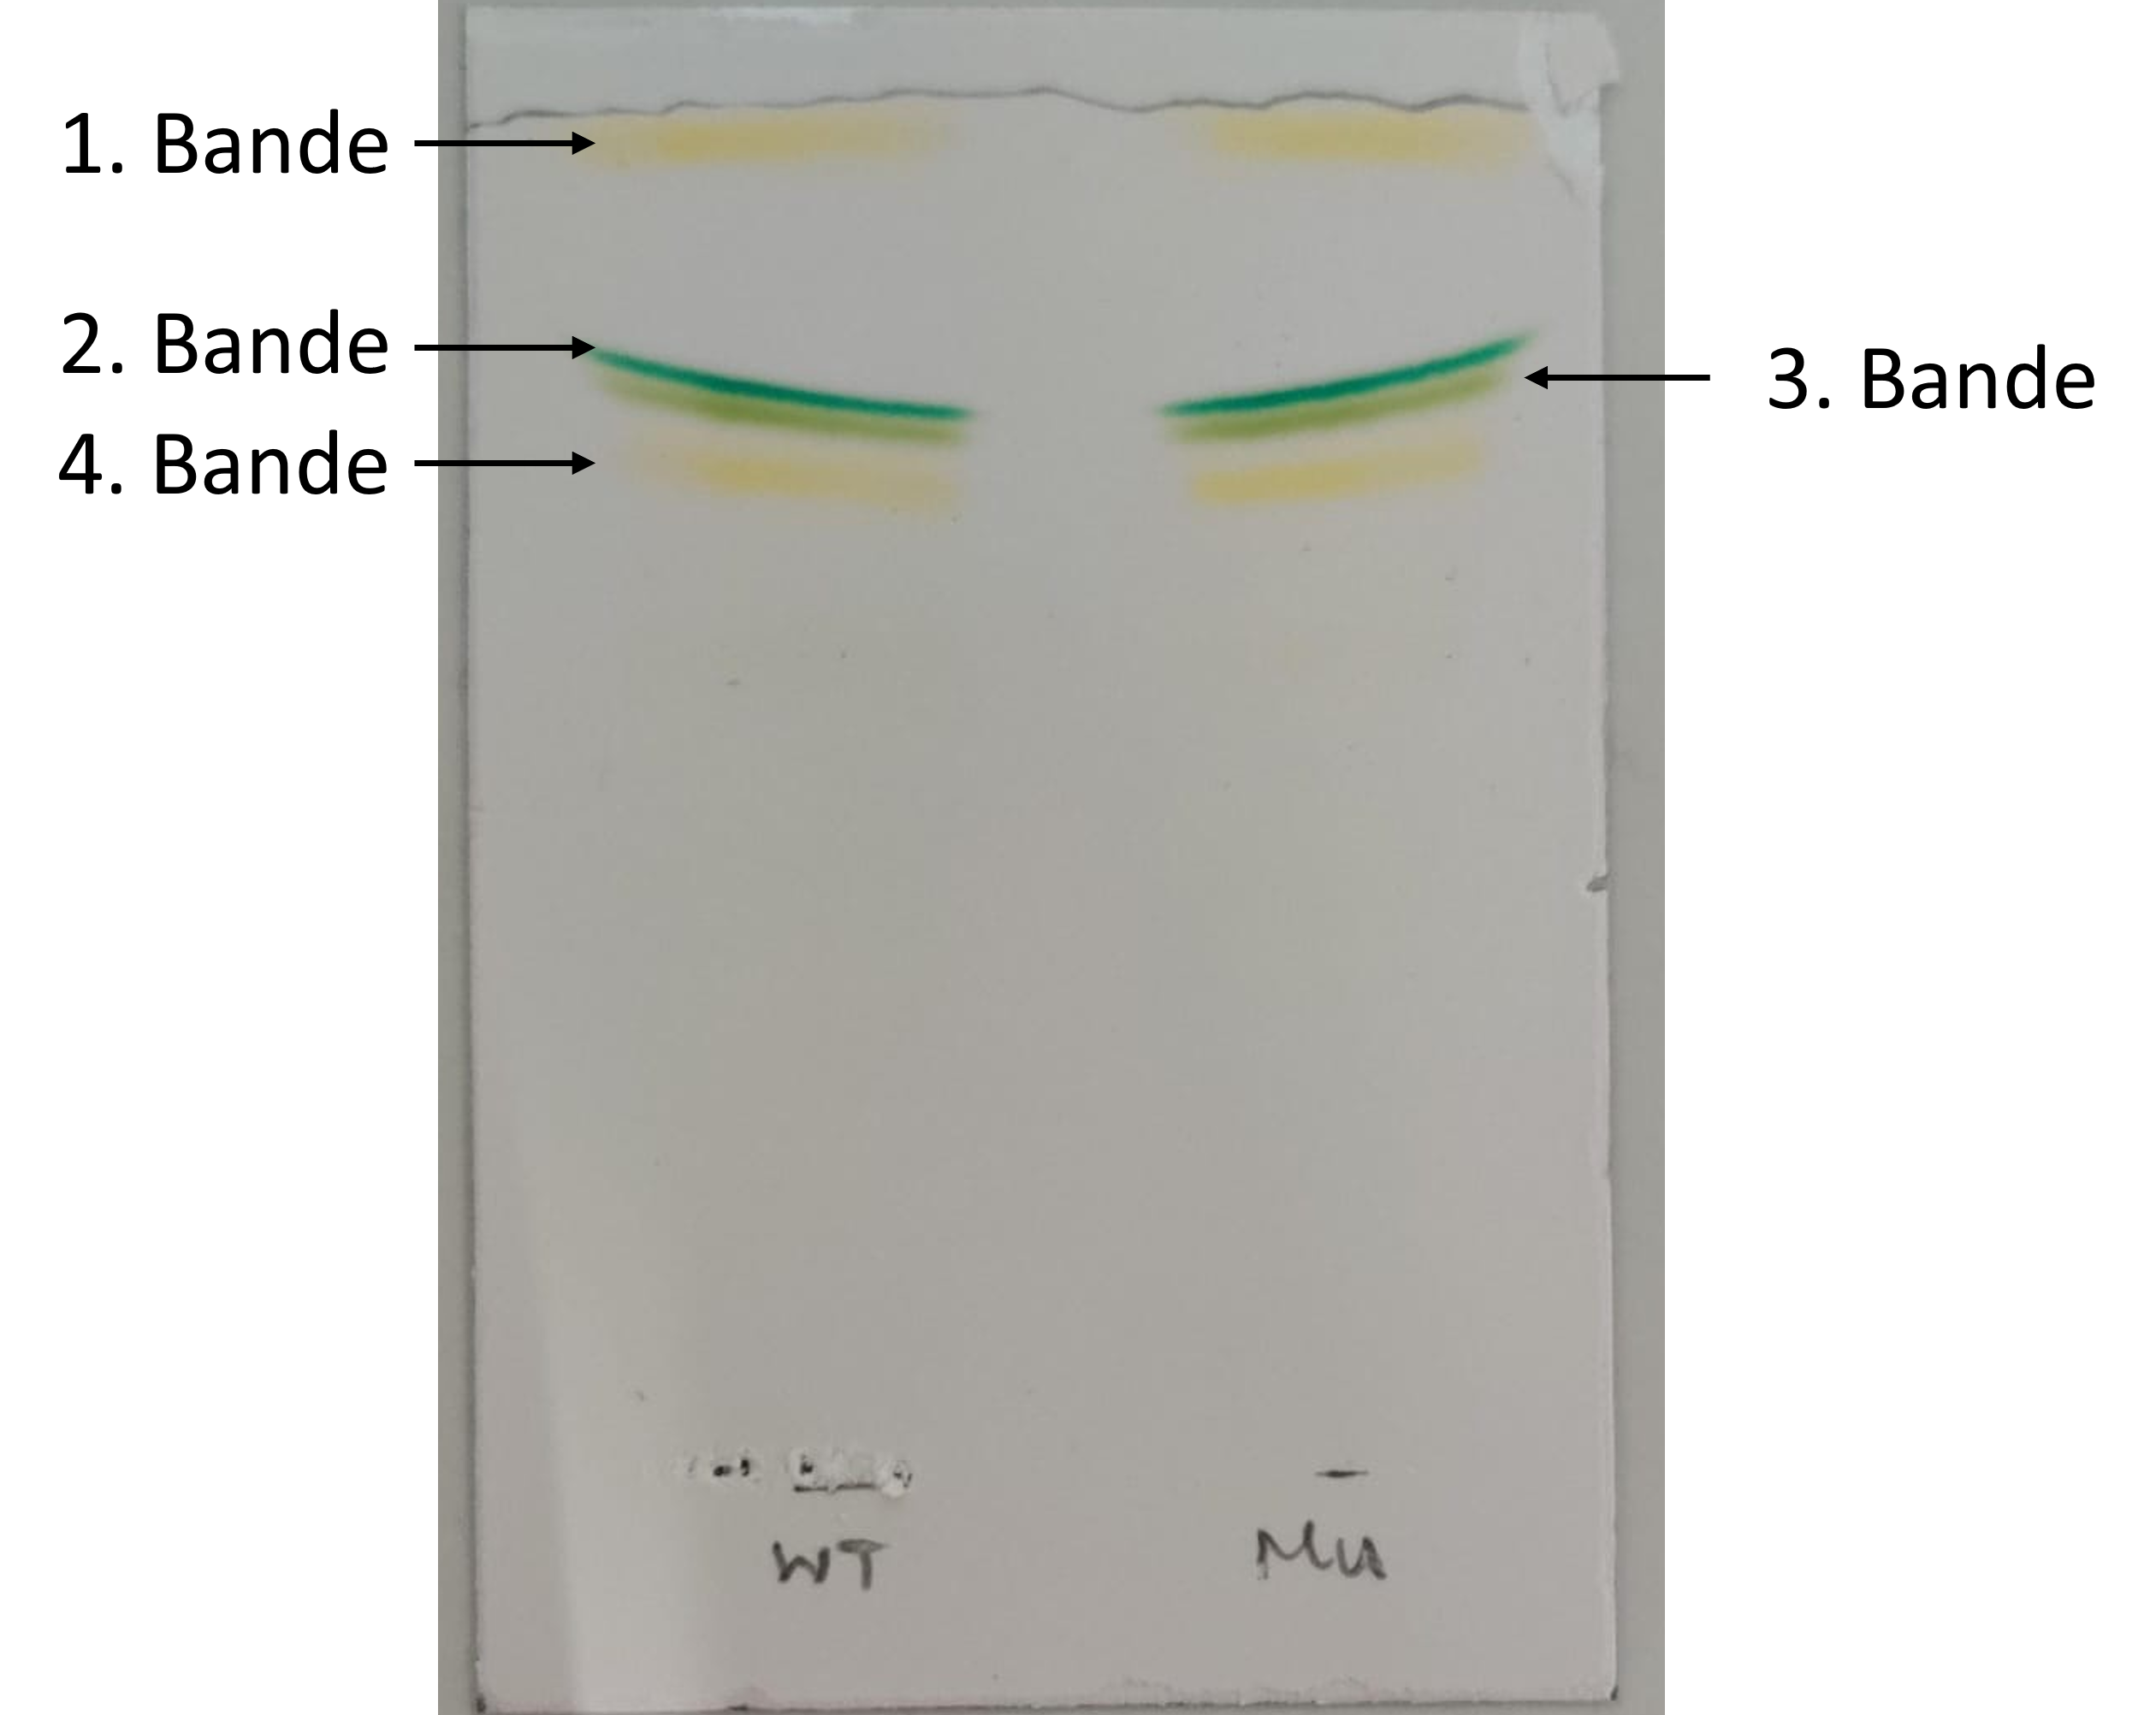
\includegraphics[scale=0.65]{DC-Plate_with_label.png}
				\caption{Probenauftrennung mittels Dünnschicht Chromatographie-Platte von der Spezies Nicotina tabacum (Wildtyp und FC1 - Mutant). Pigment wurden in Petrolether überführt und auf die Platte aufgetragen.}
				\label{fig:DC_Platte}
			\end{figure}
		
		Auf der DC-Platte sind 4 stark gefärbte Banden (siehe Figure \ref{fig:DC_Platte}) beim Wildtyp und Mutant zu sehen. Für die Quantifizierung der Banden wurde der R$_f$-Wert nach Gl. \ref{eq: rf_rechnung} bestimmt und die Werte in .Tab \ref{tab:Rf_wert} zu sehen sind\\
		\\
		\begin{equation}\label{eq: rf_rechnung}
			R_f = \frac{Substanzstrecke}{Laufmittelfront}
		\end{equation}
		\\
		Band 1 und 4 sind gelblich gefärbt und Band 2 und 3 grünlich, wobei die dritte Bande hellgrün gefärbt ist.\\
		
			\begin{table}[H]
				\centering
				\caption{$R_f$-Werte von Band 1-4 aus Figure \ref{fig:DC_Platte} vom Nicotina Tabacum Wildtyp und Mutant.}
				\label{tab:Rf_wert}
				\begin{tabular}{ccc}
					\toprule
					Band&Wildtyp& Mutant\\
					\midrule
					1& 0.97 & 0.97\\
					2 & 0.79 & 0.79\\
					3 & 0.73 & 0.73 \\
					4 & 0.61 & 0.61\\
					\bottomrule
				\end{tabular}
			\end{table}	
			
			Das Absorptionsverhalten der Bande 1 zeigt ein stark verrauschte Kurve, wo der Absorptionsmaximumbereich ungefähr bei $\lambda$ = 420 - 460 nm (siehe Figure \ref{fig:erste Bande}) liegt.\\
			Bande 2 besitzt zwei Absorptionsmaxima bei $\lambda$ = 430 und 664 nm (siehe Figure \ref{fig:zweite Bande}) und zusätzlich zwei kleinen Peak bei  $\lambda$ = 412 nm und 614 nm.\\
			In Figure \ref{fig:dritte Bande}  besitzt die Substanz der Bande 3 ebenfalls mehr als zwei Absorptionsmaxima. Zwei Absorptionsmaxima sind bei $\lambda$ = 458 und 646 nm und ein weiteren kleinen Peak bei $\lambda$ = 434 nm.\\
			Die Absorptionskurve von Bande 4 ist wie von Bande 1 etwas verrauscht und hat zwei Peaks bei $\lambda$ = 448 und 476 nm (siehe Figure \ref{fig:vierte Bande}).\\
			Bei den vier Absorptionsspektrum (Figure \ref{fig:erste Bande} - \ref{fig:vierte Bande}) existiert ein kleiner Peak bei $\lambda$ = 540 nm.\\
			Die vom Betreuer gegebene Pigmentextraktes zeigt mehrere Peaks (siehe Figure \ref{fig:fünfte Bande}), welches bei der Überlappung mit Bande zwei und drei Gemeinsamkeiten der Absorptionsmaxima zeigen (Siehe Figure \ref{fig:kombinierteabsorptionsspektrum}). Ein Peak jedoch ist beim Pigmentxtrakt nicht zu sehen, welches bei Bande 3 zu sehen ist. Der Peak bei $\lambda$ = 646 nm wurde in Figure \ref{fig:kombinierteabsorptionsspektrum} rot hervorgehoben.\\
			Die Signalintensität des Pigmentextraktes ist circa 3 mal höher als die von Band 2 und 3.
			
			
			\begin{figure}[H]
				\centering
				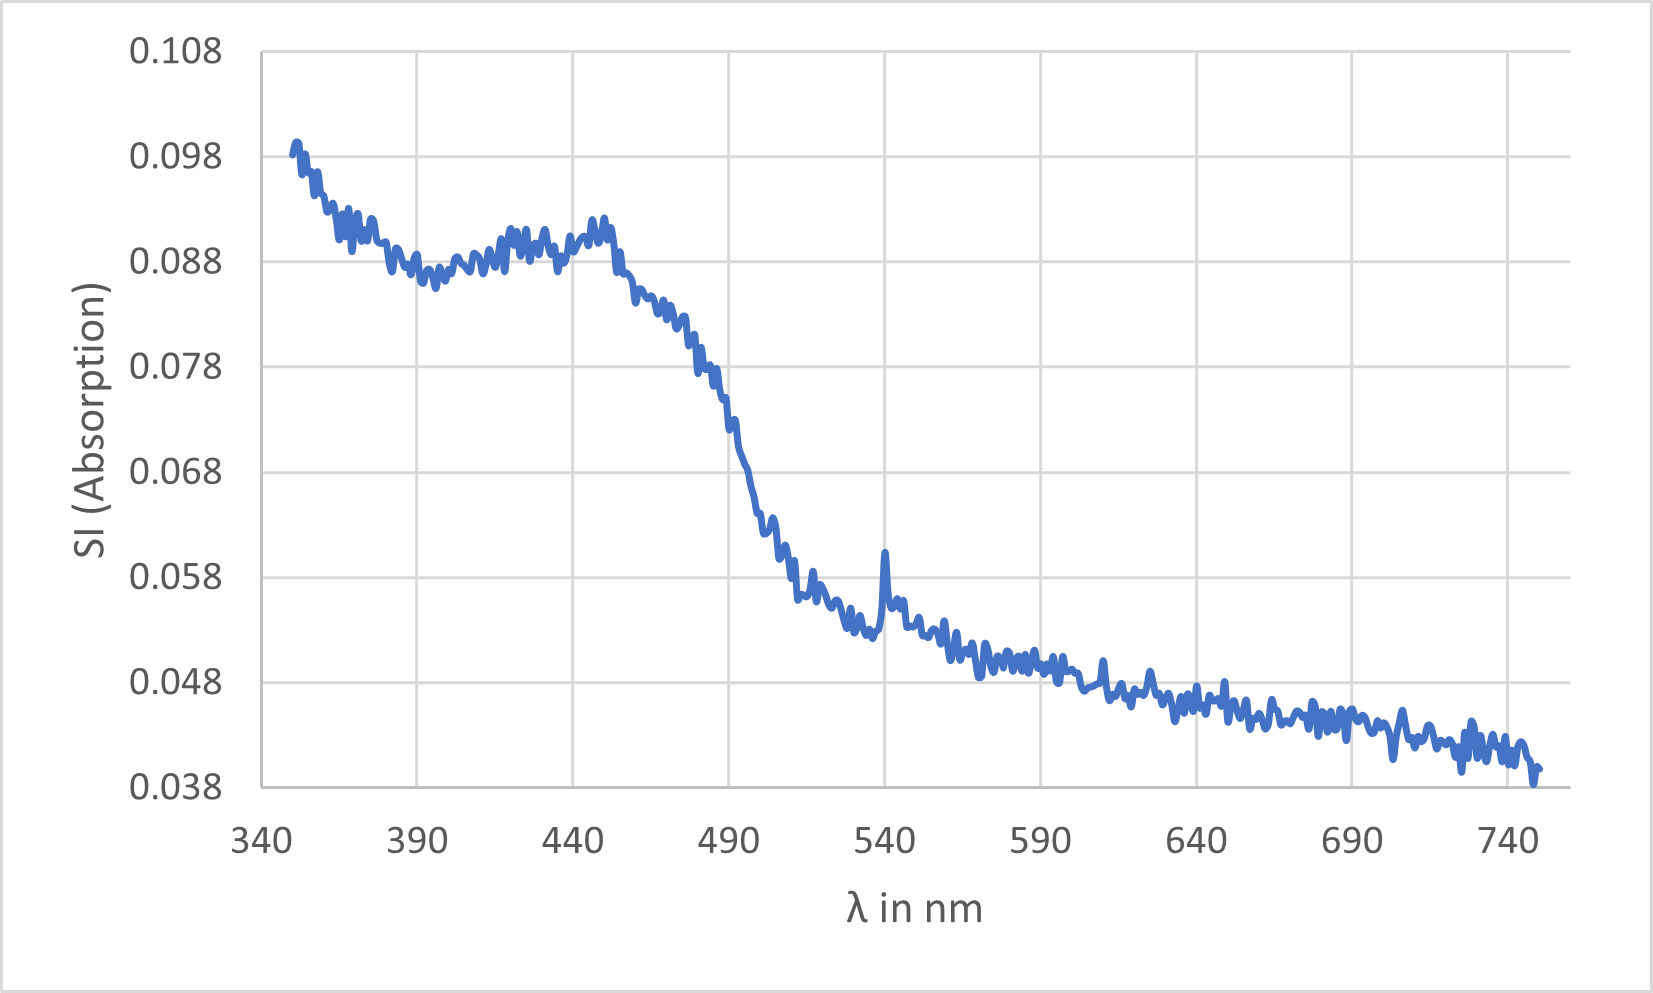
\includegraphics[scale=1]{firstband_axischange.png}
				\caption{Absoprtionsspektrum der ersten Bande aus Figure \ref{fig:DC_Platte}. Absorptionsmaxima liegt bei $\lambda$ = 420 bis 460 nm.}
				\label{fig:erste Bande}
			\end{figure}
			
			\begin{figure}[H]
				\centering
				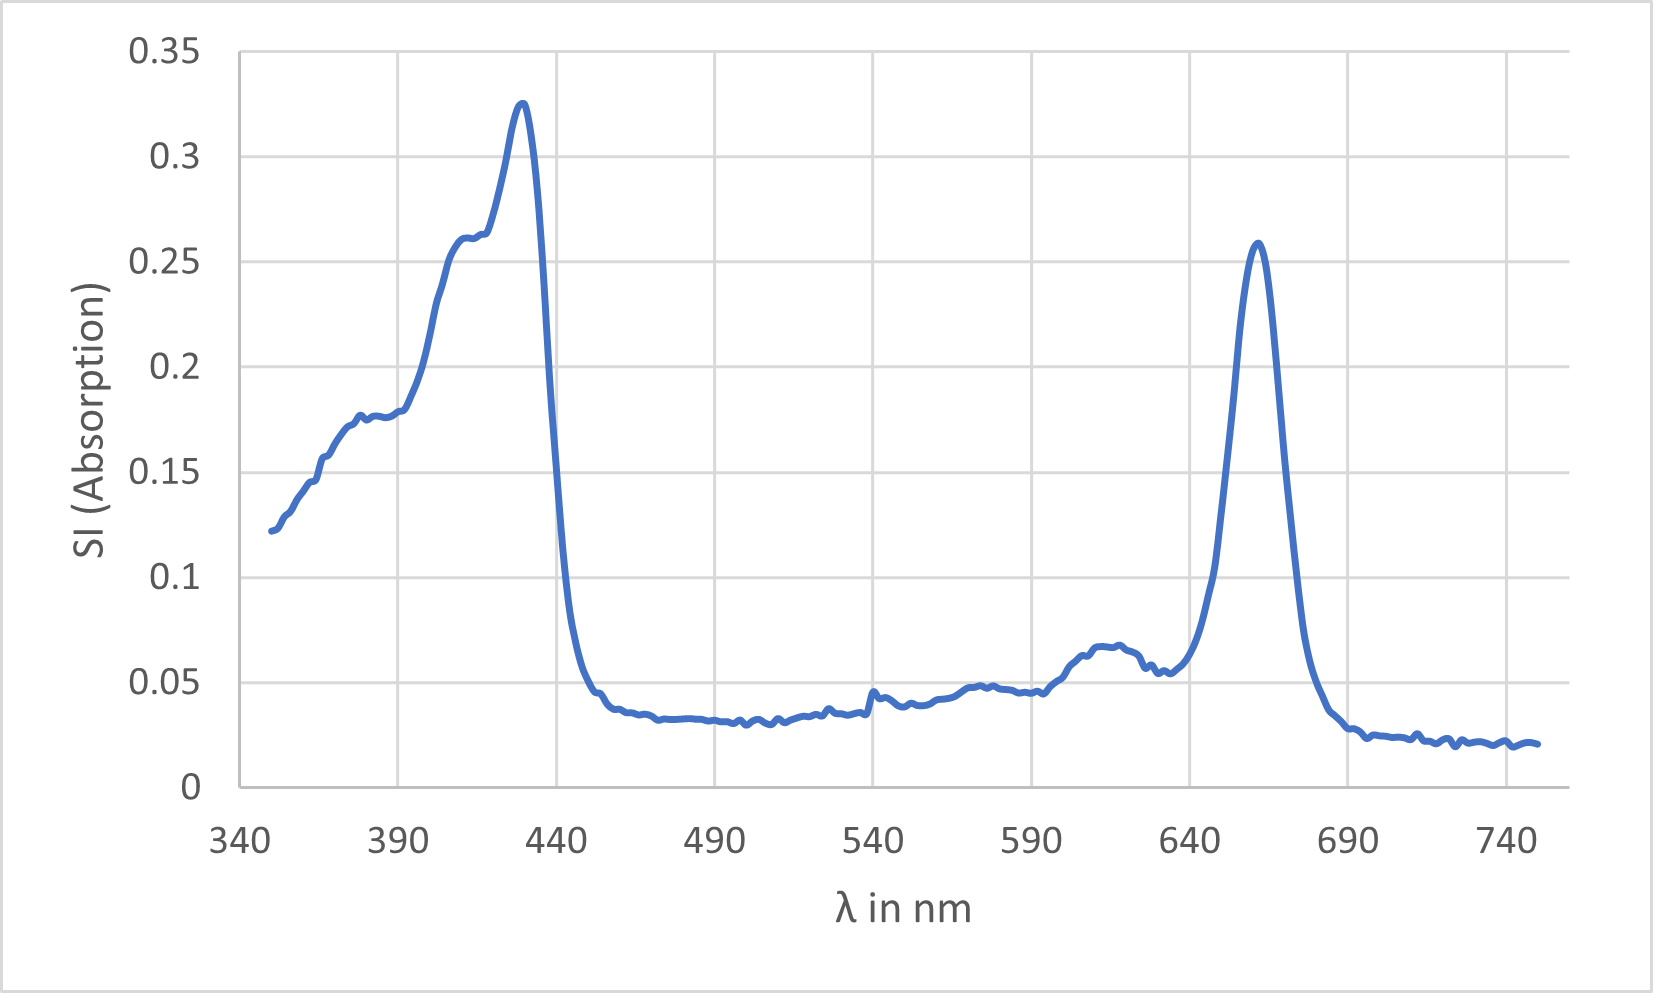
\includegraphics[scale=1]{secondband.png}
				\caption{Absoprtionsspektrum der zweiten Bande aus Figure \ref{fig:DC_Platte}. Absorptionsmaxima Bereich liegt im Bereich $\lambda$ = 430 und 664 nm.}
				\label{fig:zweite Bande}
			\end{figure}
			
			\begin{figure}[H]
				\centering
				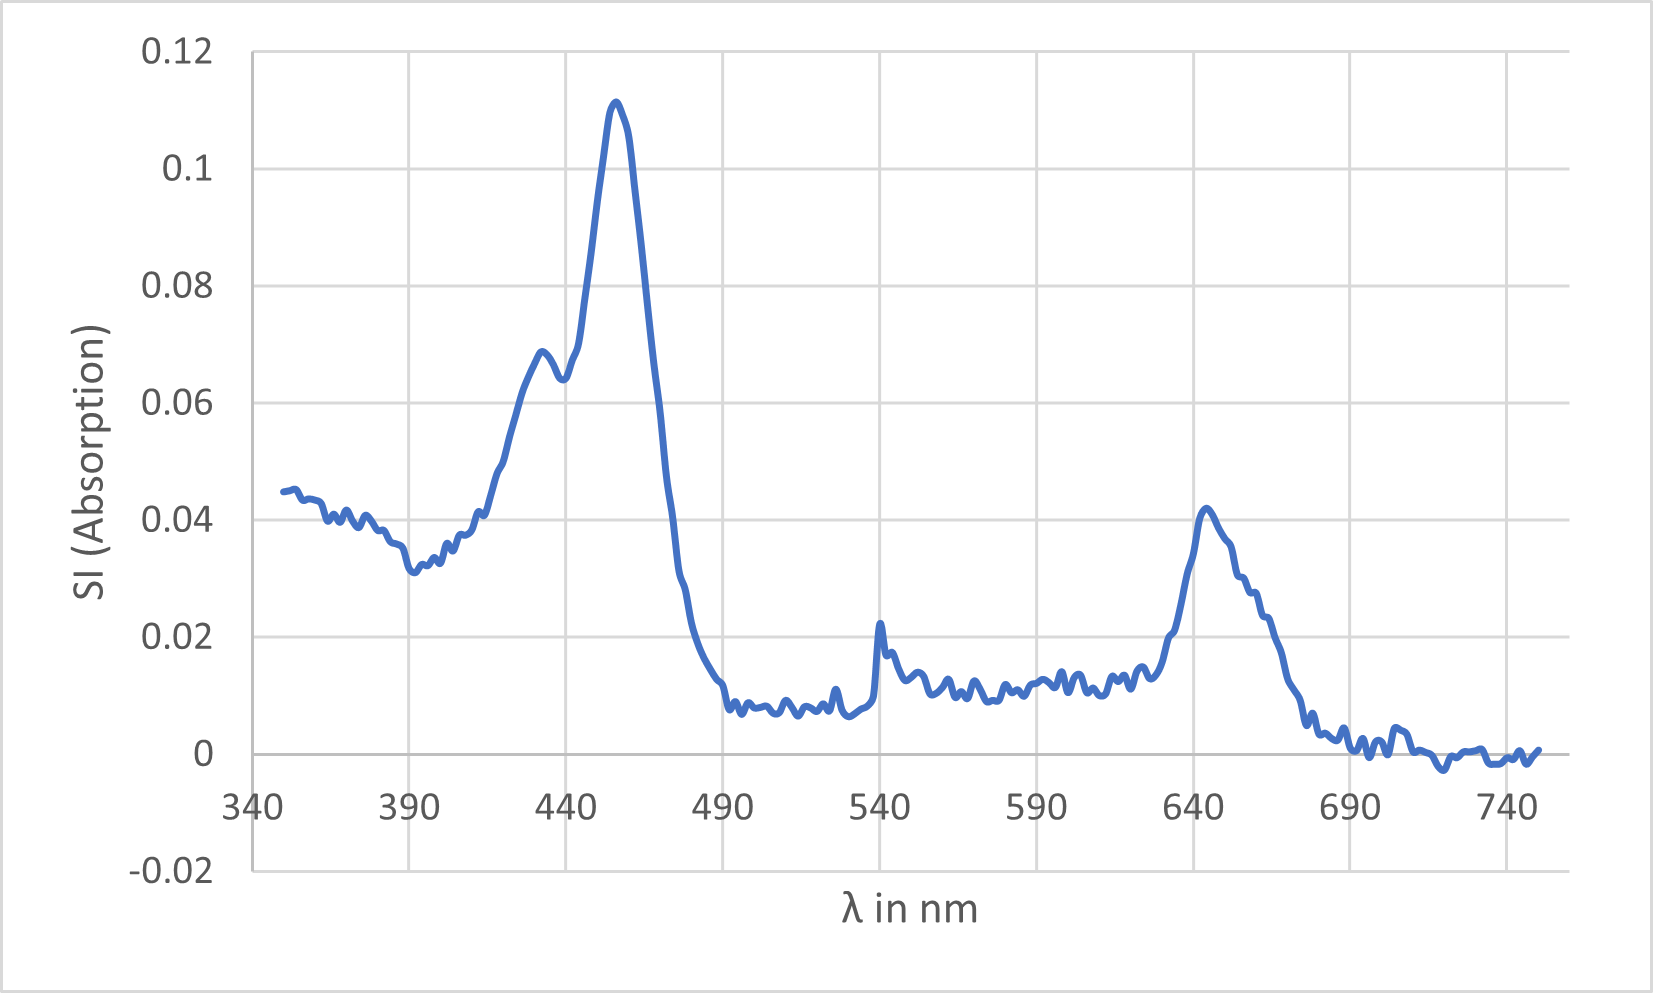
\includegraphics[scale=1]{thirdband.png}
				\caption{Absoprtionsspektrum der dritten Bande aus Figure \ref{fig:DC_Platte}. Absorptionsmaxima Bereich liegt im Bereich $\lambda$ = 458 und 646 nm. In diesen Absorption gibt es ein weiteren Peak bei $\lambda$ = 434 nm}
				\label{fig:dritte Bande}
			\end{figure}
			
			\begin{figure}[H]
				\centering
				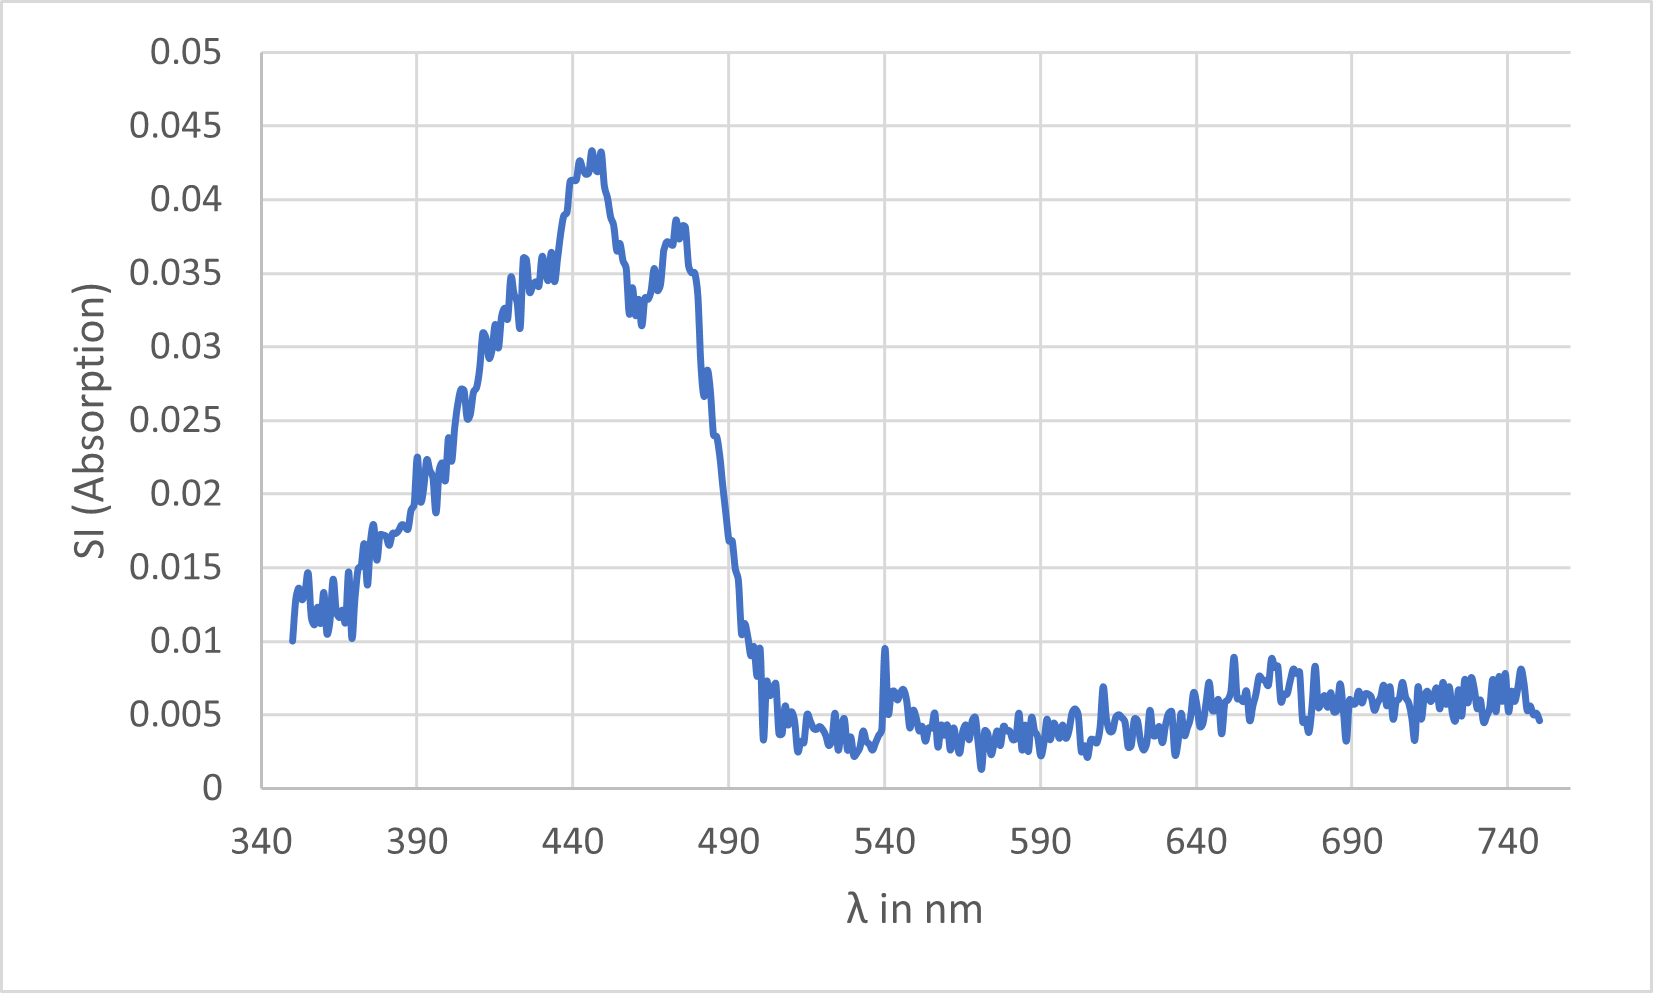
\includegraphics[scale=1]{fourthband.png}
				\caption{Absoprtionsspektrum der vierten Bande aus Figure \ref{fig:DC_Platte}. Absorptionsmaxima Bereich liegt im Bereich $\lambda$ = 448 und 476 nm.}
				\label{fig:vierte Bande}
			\end{figure}
			
			\begin{figure}[H]
				\centering
				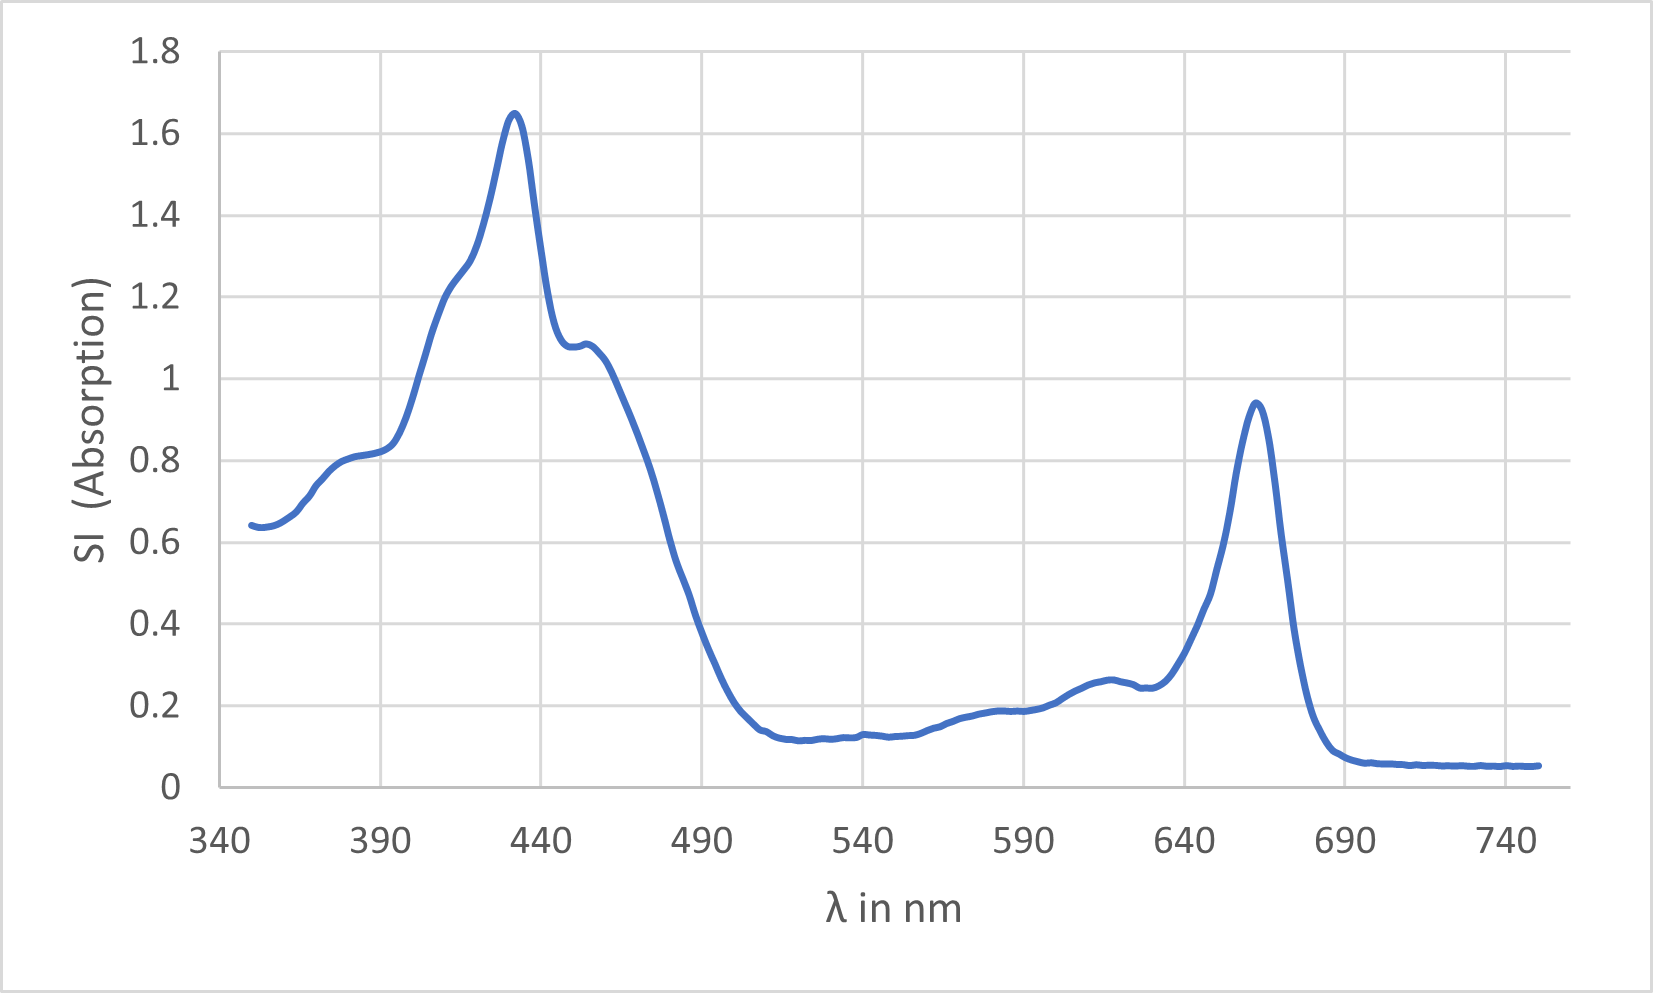
\includegraphics[scale=1]{fifthband.png}
				\caption{Absoprtionsspektrum vom Pigmentextraktes, welches der Betreuer uns mitgegeben hat.}
				\label{fig:fünfte Bande}
			\end{figure}
			
			\begin{figure}[H]
				\centering
				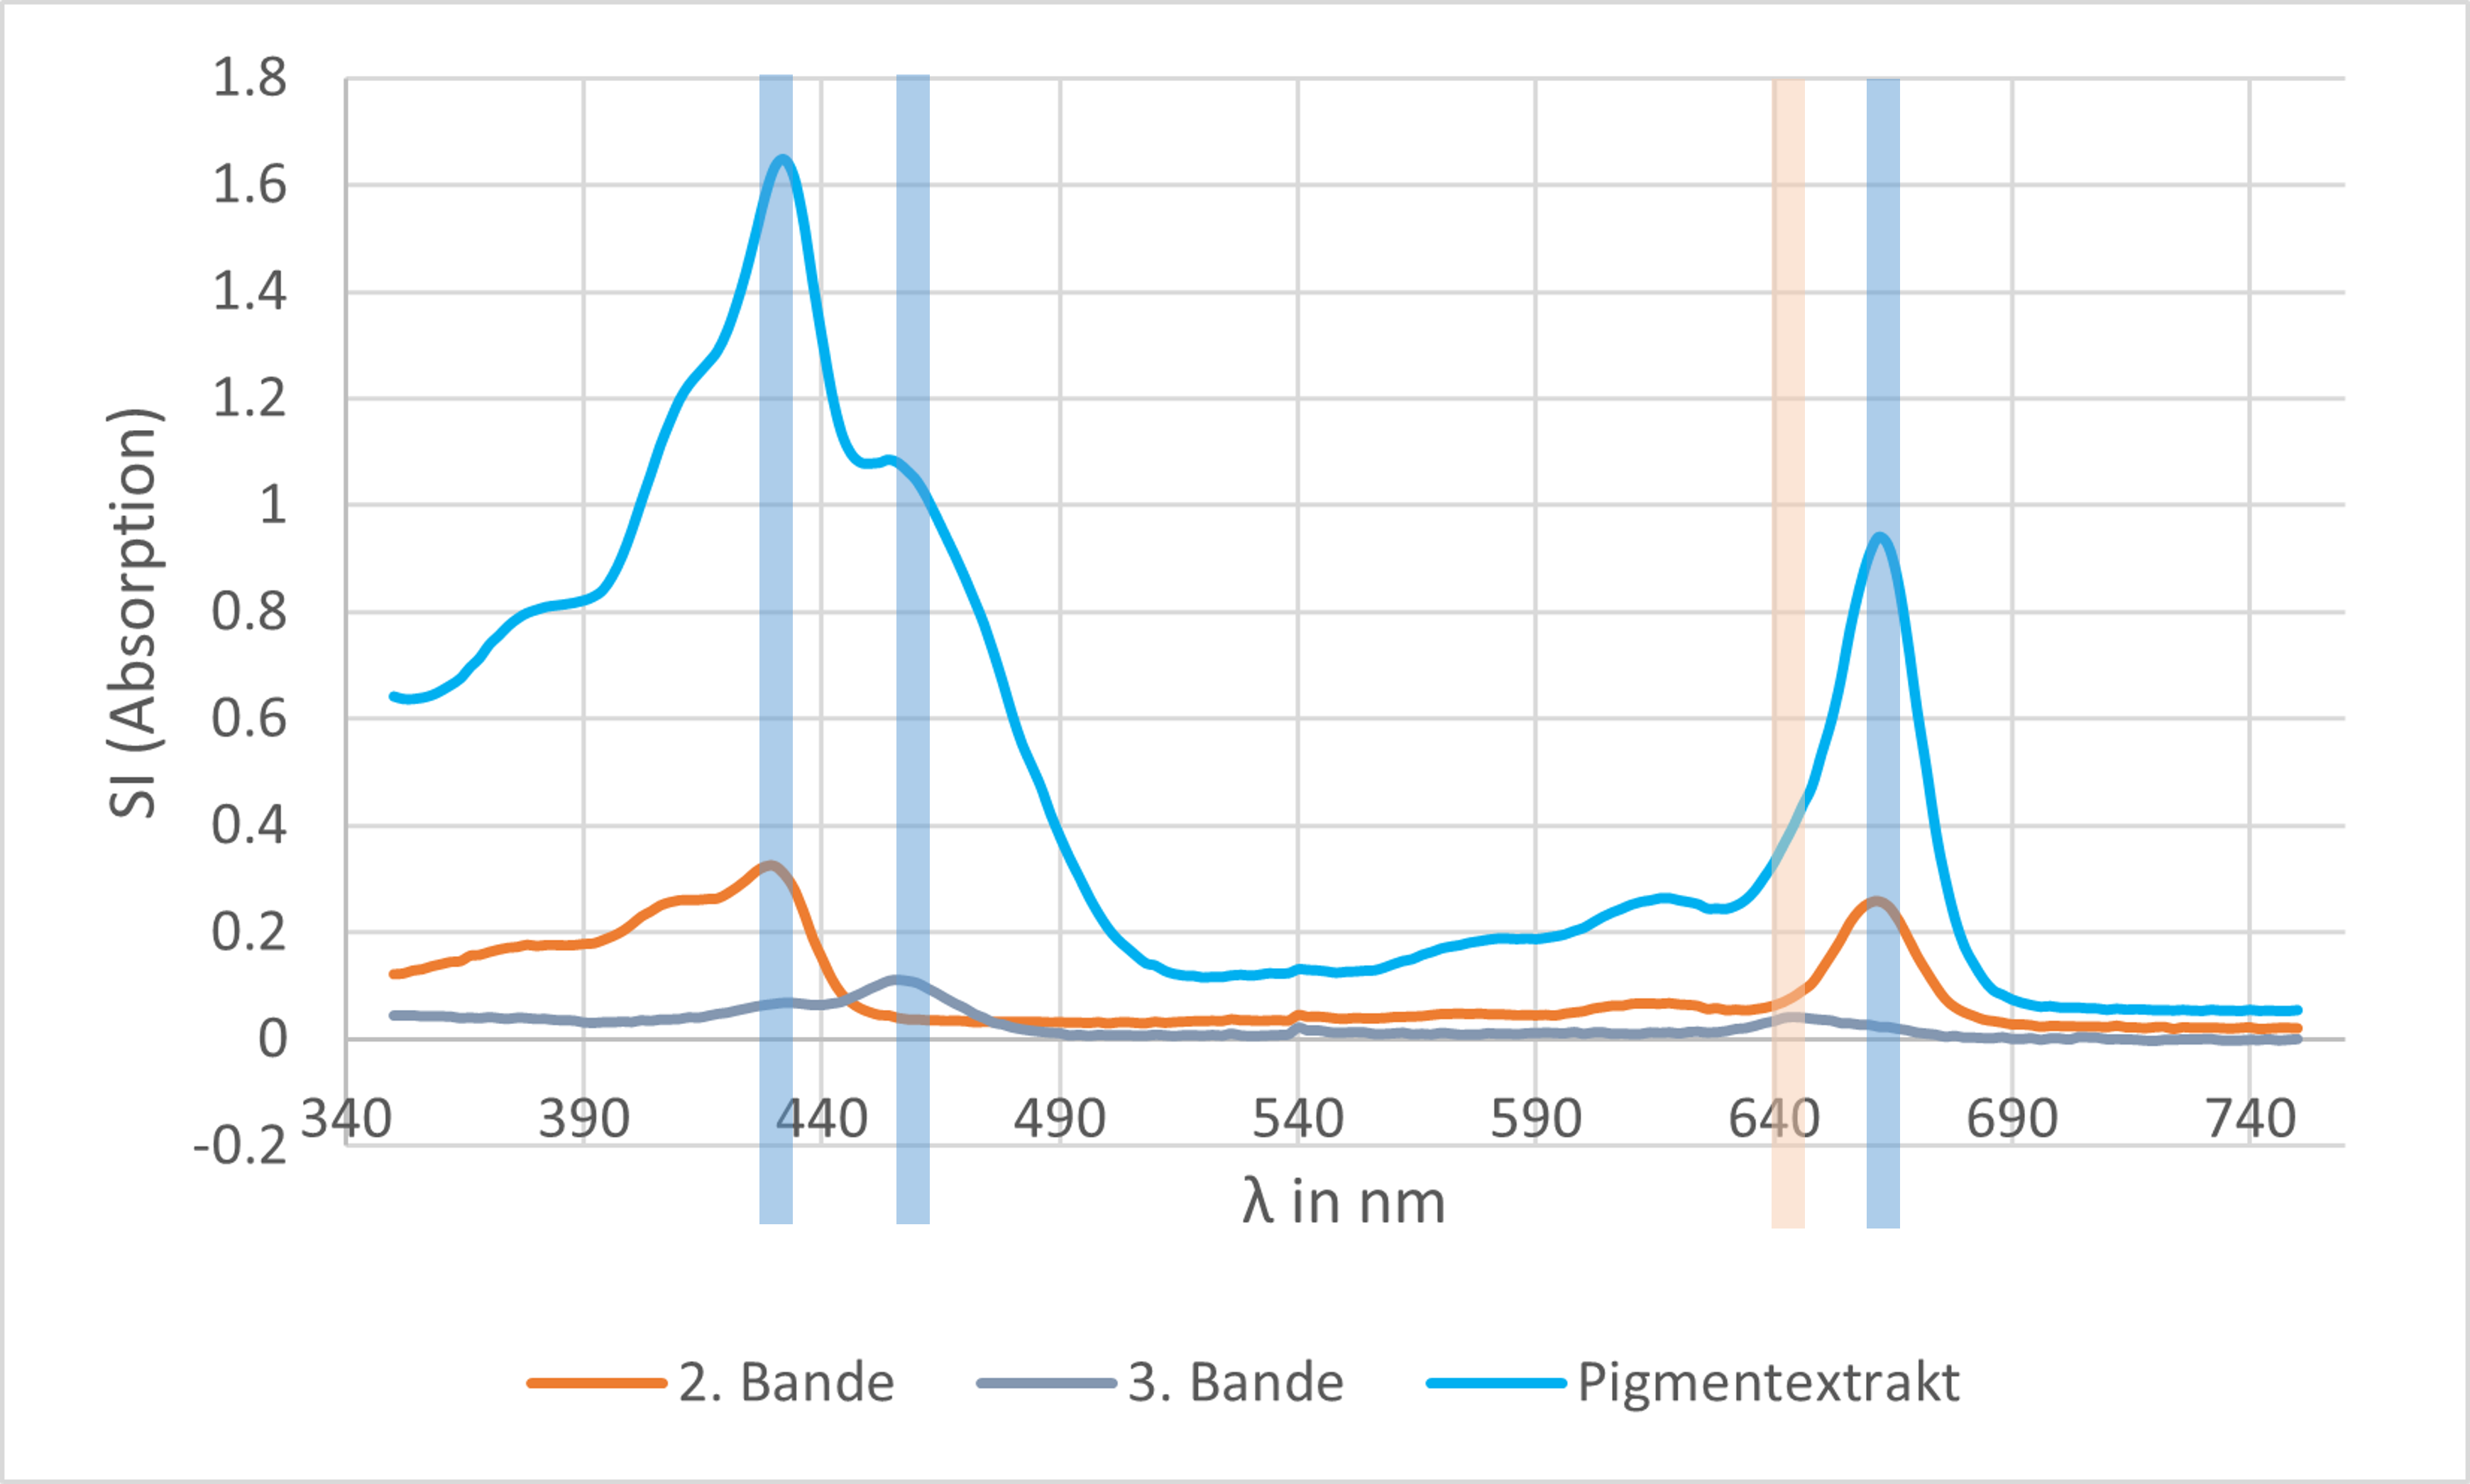
\includegraphics[scale=0.5]{combinedwithcommonpeaks_Pigmentextrakt.png}
				\caption{Vereintes Absorptionsspektrum von der unbekannten Probenextraktes, der zweiten und dritten Bande. Die Maximas der zweiten und dritten Bande wurde hier farblich hervorgehoben. Die rote Markierung zeigt ein fehlenden Peak bei der unbekannte Probeextraktes}
				\label{fig:kombinierteabsorptionsspektrum}
			\end{figure}
			
		\subsection{Fluoreszenzmessung des Pflanzenextraktes}
		
			\begin{figure}[H]
				\centering
				\includegraphics[scale=0.5]{Fluoreszenzbild}
				\caption{Fluoreszenzverhalten des Chlorophylls in Gegenwart von UV-Licht vom Wildtyp und Mutant in Petrolether und Wildtyp in wässrigen Lösung}
				\label{fig:Fluoreszenzbild}
			\end{figure}
			
		In Figure \ref{fig:Fluoreszenzbild} ist zu erkennen, dass die mit Petrolether versetzen Extrakte rot leuchten und das wässrige Extrakt nicht leuchtet, bzw. keine Verfärbung aufweist. 
		
		\subsection{Phäophytinbildung}
			Durch Zugabe von schon einem Tropfen Salzsäure zum Petroletherextrakt des Wildtyps konnte eine bräunliche Verfärbung an der Oberfläche des Extrakts erkannt werden. Durch Schütteln des Extrakts verfärbte sich das gesamte Extrakt in ein schmutziges Dunkelgrün. Auch beim Petroletherextrakt der Mutante konnte eine Verfärbung beobachtet werden, die der des Wildtyps glich. \\
				
	\section{Diskussion}
		Aus der Nicotina Tabacum Pflanze wurde von der FC1-Antisense Mutante mehr Chlorophylle a und b als beim Wildtyp extrahiert(siehe Table \ref{tab:konzentration chl a und b}).\\
		Das Verhältnis zwischen Chl a und Chl b bei beiden Pflanzentypen sind gleich. Chl a ist 1.5 mal mehr konzentriert als Chl b.\\
	
		
		\subsection{Quantifizierung Photosynthesepigmente}
			In Figure \ref{fig:DC_Platte} ist zu erkennen, dass beim Wildtyp und Mutant die vier Banden jeweils die gleichen R$_f$-Werte besitzen. Eine Farbintensitätsunterschied zwischen den beiden wird nicht beobachtet, was auch daran liegen kann, dass die eingesetzte Konzentration bei beiden unterschiedlich waren. (Vom Mutant liegt die Chlorophyllkonzentration 1.5 mal höher).\\
			Bei der Extraktion der Pigmente in den Banden wurde angenommen, dass es sich bei Mutant und Wildtyp sich um die gleiche Substanz handelt und diese somit vereint werden konnte um das Absoptionsspektrum mit eine gute Signalintensität beobachtet werden kann.\\
			\\
			Farblich gesehen handelt es sich bei der 2. und 3. Bande um Chlorophylle und bei der 1. und 4. Bande um eine Carotinoid-Verbindung.\\
			Chlorophylle absorbiert im roten und blauen Bereich und erscheint somit grün für das menschliche Auge. Carotinoide absorbiert im blauen Bereich und erscheint orange bis gelblich.\\
			Die Funktion des Chlorophylls ist in den Pflanzenzellen Licht zu absorbieren, Energie zu transferieren und Ladungen zu trennen und Carotinoide-Verbindungen schützen die Zellen vor oxidativenSchäden, indem sie bei zu viel Energiezufuhr diese in Wärme umwandeln (Wärmedissipation).\\
			\\
			Die DC-Trennung, welches hier verwendet wurde, um die Pigmente zu trennen, funktioniert nach der unterschiedlichen Affinität der Substanzen zu einer stationäre Phase. In diesen Versuch ist die stationäre Phase ein polares silikatbeschichtete DC-Platte.\\
			Je polarer ein Substanz ist, desto früher bleibt diese an der stationären Phase hängen(es wird adsorbiert). Das Laufmittel bzw. mobile Phase ist in diesen Versuch ein stark unpolares organisches Lösungsmittel (Petrolethergemisch,siehe Abschnitt \ref*{text: DC}), dass durch Kapillarkräfte die DC-Platte durchzieht und dabei das Substanzgemischt mitzieht.\\
			\\
			Chl a besitzt an ihren Tetrapyrrolring eine Methylgruppe und Chl b an der selben Position eine Aldehydgruppe. Somit ist Chl b polarer und hat eine größere Affinität zur stationären Phase als Chl a und läuft somit langsamer.\\
			Anhand des Absorptionsspektrum ist zu erkennen, dass Bande 2 zwei Peaks bei $\lambda$ = 430 und 664 nm besitzt und diese mit Peter von Sengbusch gemessenen Absorptionsspektrum für Chl a übereinstimmt (Literaturwert ist $\lambda$ = 430 und 662 nm\cite{Absorption_Maxima_Chlorophylle} ).\\
			Chl b hat sein Absorptionsmaxima bei $\lambda$ = 453 und 642 nm\cite{Absorption_Maxima_Chlorophylle} und gemessen wurde hier bei $\lambda$ = 458 und 646 nm.\\ 
			In der Kurve in Figure \ref{fig:dritte Bande} ist ein kleiner Peak bei $\lambda$ = 434 nm zu erkennen, dass höchstwahrscheinlich von der zweiten Bande kam. Da beide Banden relativ nah gelaufen sind, ist die Kontaminationsgefahr relativ hoch.\\
			Dadurch dass die Absorptionsmaxima von Chl a und b verschieden sind, kann diese auch bei Kontamination differenziert werden.\\
			Diesen Vorteil nutzen die Pflanzen auch, um das rote Licht energetisch maximal zu verwerten.\\
			\\
			Bei den restlichen zwei Banden handelt es sich um carotinoidische Verbindungen.
			Die erste Bande musst eine Substanz sein, das sehr unpolar ist. ß-Carotin ist von den Carotinoide das unpolarste Molekül.\\
			Das Absorptionsspektrumsverhalten von ß-Carotin ähnelt den von A.Hager gemessenen Werten $\lambda$ = 451 und 478nm\cite{Absorption_Maxima_Carotinoide}. Da die Kurve in Figure \ref{fig:erste Bande} sehr verrauscht ist, können die beiden Absorptionsmaxima nicht genau abgelesen werden. Die Peaks lieben ungefähr in den Bereich $\lambda$ = 420 bis 460 nm. Aber aufgrund des Laufverhalten in der DC wird vermutet, dass es sich bei der 1. Bande um ß-Carotin handelt.\\
			Die 4. Bande ist polarer also die restlichen Photosynthesepigmenten.  Nach A.Hager könnte es sich hier um das Carotinoid Lutein handeln, dass sein Absorptionsmaxima bei $\lambda$ = 446 und 474\cite{Absorption_Maxima_Carotinoide} nm. \\
			\\
			Zusätzlich wurde vom Betreuer ein Rohextraktprobe mitgegeben, dessen Absorptionsspektrum ebenfalls aufgenommen wurd.\\
			Das Absorptionsspektrum wurde mit den Absorptionsspektrum des Chlorophylls vergliechen (siehe Figure \ref{fig:kombinierteabsorptionsspektrum}).\\
			Die Rohextraktprobe zeigt ein kombiniertes Absorbtionsverhalten von Chl a und b, mit eine kleine Ausnahme bei  $\lambda$ = 642 nm . Dort fehlt dem Rohextraktes den Peakt im rotwelligen Bereich\\
			\\
			Der Versuch zeigt, dass die Photosynthesepigmente mittels DC aufgetrennt werden kann. Die Zuordnung der einzelnen Pigmenten zu den Substanzen kann nicht alleine durch das Absorptionsspektrum charakterisiert werden und könnte bei der DC-Trennung mit einem Referenzsubstanz besser quantifiziert werden. Die Carotinoide zeigen untereinander ein relativ ähnliches Absorptionsverhalten, jedoch mit parallel laufenden Referenzsubstanzen kann die Polarität noch ein Charaktiriesierungsmerkmal sein. ß-Carotin konnte als einzige aufgrund der unpolaren Struktur gut identifiziert werden\\
			Für eine bessere Bandenauftrennung, insbesondere von Chl a und b, könnte der Lauf zusätzlich verlängert werden.\\
			\\
		
		\subsection{Fluoreszenzverhalten von Chlorophylle}
			Zu das Fluoreszenzverhalten von Chlorophylle in Figure \ref{fig:Fluoreszenzbild}.
			Das rote Leuchten der Petroletherextrakte kann man als Fluoreszenz deuten. Um zu verstehen, warum man eine Fluoreszenz bei dem Petroletherextrakt beobachten kann ist, muss man verstehen, warum Blätter nicht fluoreszieren, wenn man sie mit einer UV-Lampe bestrahlt, obwohl sie natürlich Chlorophyll enthalten. Nun, solange sich Chlorophyll im Blatt befindet, erfüllt es seine Funktion als Pigment im Photosystem I und II, kann also durch die energetische Anregung als Energiedonor dienen. Wird es, wie in diesem Experiment durchgeführt, aus den Pflanzenzellen extrahiert, dann kann man eine Fluoreszenz unter dem UV-Licht beobachten. Das Petroletherextrakt sorgt dafür, dass die Photosysteme zerstört werden und die von den Chlorophyllen aufgenommenen Photonen nicht auf das restliche Photosystem übertragen werden, sondern direkt wieder reflektiert werden. \\
			\\
			Zwischen dem Wildtyp und der Mutante sind keine auffäligen Unterschiede in der UV-Licht-induzierten Färbung zu erkennen. Jedoch könnte man bei der Mutante, aufgrund des Vorhandenseins des 35S-Promotors, vermuten, dass die Färbung weniger stark intensiv rot ist. Da p35S ein antisense Promotor für FC1 ist, würde dies eine Runterregelung von Chlorophyll bedingen. Warum ist dies nun mit einer verringerten Färbung zu assoziieren, also was bedeutet Chlorophyllfluoreszenz?\\
			Chlorophyll a und b haben je zwei Absorptionsmaxima, je eines im Bereich der blauen und roten Wellenlängen des sichtbaren Lichtes. Chlorophyll a absorbiert im blauen Bereich (430-450 nm), mit einem Peak bei 430 nm und im roten Bereich (640-680 nm), mit einem Peak bei 662 nm. Chlorophyll b absorbiert auch im auch im blauen und roten Bereich, jedoch bei Wellenlängen von 450-500 nm und 640-660 nm, mit Peaks bei 453 nm und 642 nm. \\
			Es verbleibt ein Bereich des Spektrums zwischen 490 und 620 nm im grüner Wellenlängenbereich, der nicht absorbiert wird und stattdessen reflektiert wird, auch „die Grünlücke“ genannt, welche die charakterisierende grüne Farbe von Pflanzen hervorruft. 
			Die oben behandelte Absorption von sichtbarem Licht wird zudem begleitet von einer Emission, bzw. Fluoreszenz von Schwachlicht im längerwelligen Bereich, hauptsächlich erzeugt durch angeregte Chlorophyll-a-Moleküle im Reaktionszentrum P680 des Photosystem II. Das Niveau der Anregung von Chlorophyll ist abhängig von der Wellenlänge des Lichts: blaues Licht zum Beispeil führt zum zweiten Singulettzustand, rotes Licht hingegen verursacht den ersten Singulettzustand. Der zweite Singulettzustand kann unter Wärmeabgabe in den ersten Singulettzustand übergehen. Die Energie des ersten Singulettzustands kann für den Excitonentransfer zwischen den Chlorophyllmolekülen und im Reaktionszentrum P680 für die Elektronenübertragung auf den Primärakzeptor Q, dem “Quencher”, genutzt werden. Die  Energie kann jedoch auch durch Fluoreszenz oder Wärme in den Grundzustand zurückfallen oder in den Triplettzustand übergehen, woraufhin durch Wärmeabgabe oder Phosphoreszenz das Chlorophyll in den Grundzustand zurückkehren oder seine Energie auf Carotinoide übertragen kann. \\
			\\
			Nun, wie ist der starke Unterschied zwischen den Petroletherextrakten und dem wässrigen Extrakt zu erklären? Nun, hinleitend ist es sinnvoll zu verdeutlichen wie Phaöphytine entstehen können und was die Auswirkungen dessen sind. 
			In diesem Experiment werden zuerst durch das Mörsern die pflanzlichen Zellen grob zerstört Als Nächstes spielt das basische Aceton eine wichtige Rolle, denn es puffert die sauren Inhalte der Vakuolen. Würde der pH-Wert nicht gepuffert werden und einen Wert von 5,5 oder geringer erreichen, würden die apolaren Chlorophylle, durch Tauschen des Magnesium-Ions im aktiven Zentrum für ein Protonen, zu einem Phäophytin werden. 
			Der genaue biochemische Vorgang ist wie folgt: das aktive Zentrum von Chlorophyll besteht aus einem zentralen Magnesiumion, koordiniert durch vier Stickstoffatome in einem tetrapyrrolischen Ringsystem. Der Verlust vom Magnesiumion, bei geringerem pH-Wert, ist bedingt durch höhere Protonenkonzentration, was dazu führt, dass die Stickstoffatome im aktiven Zentrum von Chlorophyll a protoniert werden. Dadurch ist die Koordination zwischen den Stickstoffatomen und dem Magnesiumion reduziert, weshalb das Magnesiumion leichter von einem affineren Proton verdrängt werden kann. Letztendlich führt dies dazu, dass sich die Struktur, bzw. der Elektronenresonanz des Chlorophyll-Moleküls und damit das Absorptionsspektrum verändert und dadurch die Funktion und photosynthetische Effizienz vermindert.\\
			\\
			Um zurück zum Experiment zu kehren: im apolaren Medium des Petrolethers sind die Chlorophylle gut gelöst und können ihre Struktur erhalten und zeigen somit auch die charakteristische und zu erwartende Fluoreszenz. Im polaren wässrigen Medium passiert etwas Ähnliche, wie im sauren Medium (oben beschrieben): die Chlorophylle würden zu Phäophytinen und somit ihre Fluoreszenzfärbung beeinflussen. Dies spiegelt sich in den Ergebnissen wieder. 
		

		\subsection{Stabilität von Chlorophylle}
		
			Chl a und b enthalten beide ein Zentrales Magnesium-Ion im zyklisches Tetrapyrolring (siehe Figure \ref{fig:chlorophyllestruktur}).  Dieses Magnesium-Kation ist ein wichtiger Bestandteil des Chl, und trägt zu dessen spezifischen Absorptionsspektrum bei. \\
			Durch eine Ansäuerung des Mediums, wie es im Versuch mittels Salzsäure geschehen ist, lösen sich die Magnesium-Kationen sowohl aus Chl a als auch aus Chl b. Sie werden durch den Überschuss an Wasserstoffatomen aus dem Zentrum des Chl verdrängt. Statt des Magnesium-Kations binden die Stickstoff-Atome nun zwei Wasserstoffatome im Zentrum des Chl (siehe Figure \ref{fig:Phyäophytinstruktur}). Das entstandene Molekül nennt sich Phäophytin und hat nicht nur eine andere Strukturformel als Chl, sondern auch andere Eigenschaften. So hat Phäophytin eine, im Vergleich zu Chl, leicht veränderte Elektronenresonanz und damit einhergehend auch ein leicht verändertes Absorptionsspektrum. Diese Veränderung des Absorptionsspektrums wurde im Versuch sichtbar gemacht. Es kommt zu einer Veränderung der Farbe bei Chl a von blaugrün nach olivgrün und bei Chl b von gelbgrün nach bordeauxrot \cite{Chlorophyllestruktur}. Da das Petroletherextrakt sowohl Chl a als auch Chl b enthielt, mischten sich gelbgrün und bordeauxrot zu einem oliv- bis bräunlichen Ton, wie er im Versuch beobachtet wurde. \\
			Da die Vakuolen der Pflanzenzellen häufig einen sauren pH-Wert haben, ist es wichtig bei der Vorbereitung einer Probe, bei der die Photosynthesepigmente gemessen werden sollen, darauf zu achten, dass es nicht zu einer Ansäuerung des Mediums kommt. Die bei der Zerkleinerung des Rohmaterials aus den Vakuolen austretenden Säure muss deshalb mit einem basischen Puffer ausgeglichen werden, sonst würden die Chl-Moleküle schon während der Extraktion zu Phäophytin umgewandelt werden. In diesem Versuch wurde als Puffer basisches Aceton genutzt.\\
		
			
			\begin{figure}[H]
				\centering
				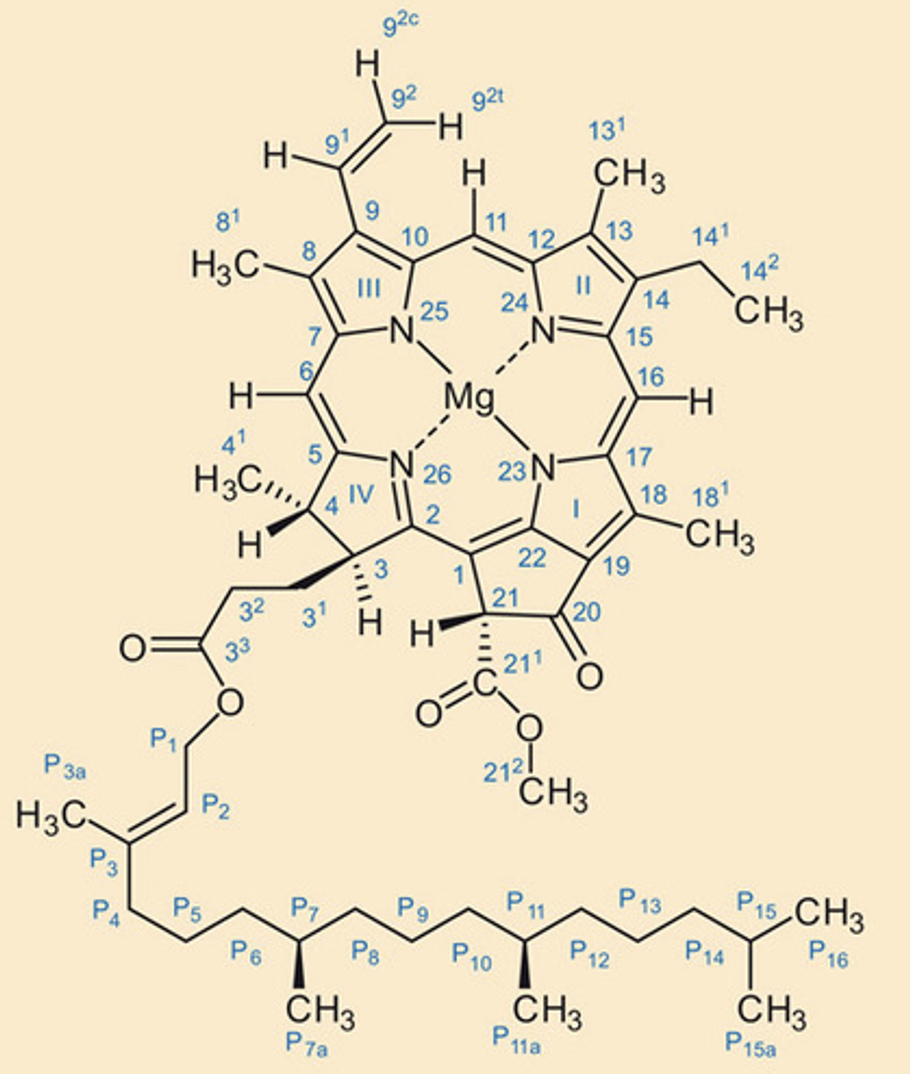
\includegraphics[scale=0.4]{Struktur_Chlorophyll}
				\caption{Strukturformel von Chl a mit Magnesium-Ion im Zentrum\cite{Chlorophyllestruktur}}
				\label{fig:chlorophyllestruktur}
			\end{figure}
			
			
			\begin{figure}[H]
				\centering
				\includegraphics[scale=0.4]{Struktur_Phäophytin}
				\caption{Strukturformel von Phäophytin a mit zwei Wasserstoff-Atomen im Zentrum\cite{Phäophytin}}
				\label{fig:Phyäophytinstruktur}
			\end{figure}
			
			Auch wenn die Umwandlung von Chl zu Phäophytin in Pflanzenzellen nicht erwünscht ist, und einen Funktionsverlust des Fotosynthesepigments bedeutet, so hat Phäophytin dennoch eine wichtige Rolle in der Elektronentransportkette des Photosystem II. So ist Phäophytin aufgrund seiner Eigenschaften ideal für die Weiterleitung von Elektronen. Aufgrund der nur leicht von Chl abweichenden Elektronenresonanz, fungiert Phäophytin als erster Elektronenakzeptor in der Kette.\\ Nachdem es zur Anregung des speziellen Chlorophyll-Paars, im Reaktionszentrum P680, durch Photonen kam, wird ein Elektron herausgelöst und an das örtlich sehr nah gelegene Phäophytin abgegeben. Dieser Prozess geschieht in wenigen Pikosekunden. Vom Phäophytin aus wird das Elektron weiter an einen Plastochinon-Komplex, bestehend aus zwei Plastochinonen, gegeben. Von hier aus wandert das Elektron weiter in der Elektrontransportkette, bis es schließlich zum Photosystem I weitergegeben wird. Im Photosystem I ist Phäophytin nicht enthalten\cite{Photosystem_phäopytin}. Phäophytin spielt also eine wichtige Rolle im Photosystem II und macht die Photosynthese möglich.\\
	
	\section{Conclusion}
	
	Interessanterweise konnte kein Unterschied an Chlorophyllekonzentration oder Verhalten zwischen der Wildtyp-pflanze und FC1-antisense-Mutante beobachtet werden.\\
	Diese wurde in den Paper von Daniel Hey \cite{FC1_Paper} ebenfalls beobachtet.
	
	\section{Anhang}
		\subsection{Rechenwege}\label{rechenwegabschnitt}
			\begin{figure}[H]
				\centering
				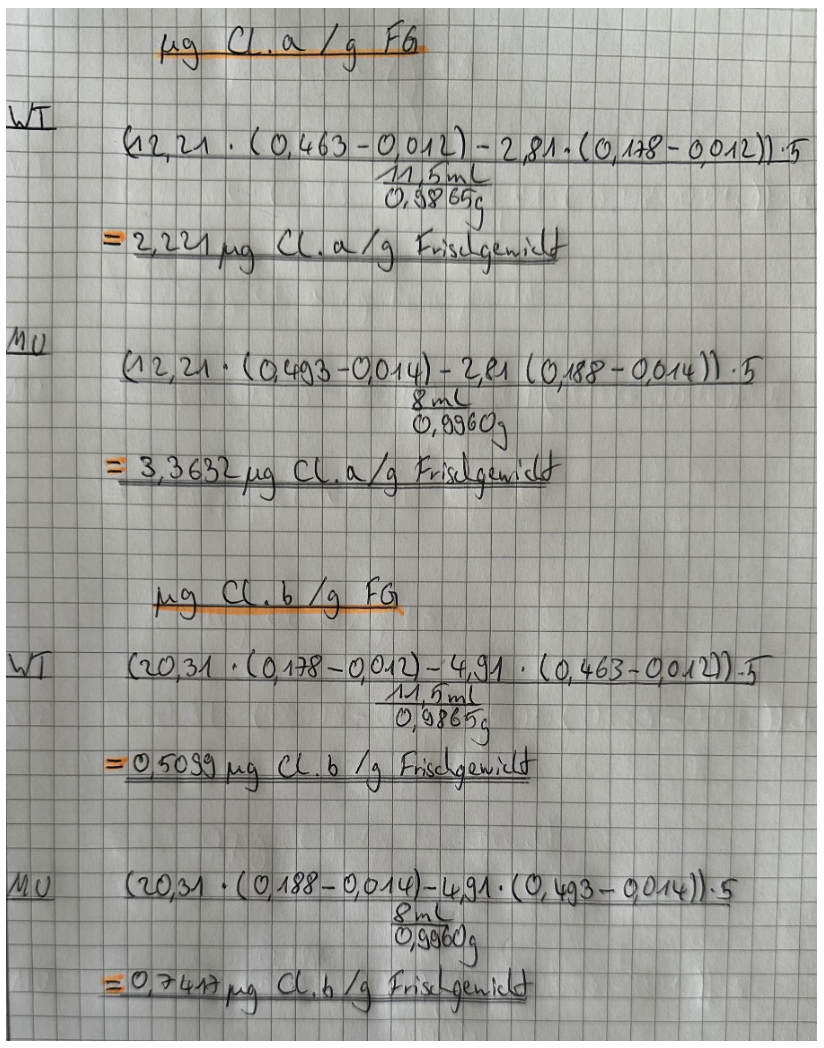
\includegraphics[scale=0.8]{Rechenweg_frido}
				\caption{Rechenweg der Konzentrationsbestimmung von Chlorophylle a und b des Rohextraktes. Absorptionswerte bei den jeweiligen Wellenlänge $\lambda$ = 470, 646, 663 und 720 nm wurde aus der Table \ref{tab:Rohdaten Extinktion Rohextraktes} entnommen.}
				\label{fig:Konzentrationsbestimmungrechenweg}
			\end{figure}
		\subsection{Rohdaten}
			\subsubsection{Einwaage der Proben }
				\begin{table}[H]
					\centering
					\caption{Masse der Blätter und das Volumen des in basischen Aceton extrahierten Pigmenten vom Nicotiana tobacum des Wildtyps und FC1-Antisense Mutant}
					\label{tab:Probemassen und Volumen}
					\begin{tabular}{ccc}
						\toprule
						&Wildtyp& Mutant\\
						\midrule
						m(Frischgewicht) in g & 0.9965 & 0.9960\\
						V(Rohextrakt) in mL & 11.5 & 8\\
						\bottomrule
					\end{tabular}
				\end{table}
				
			\subsubsection{Extinktion des Rohextraktes}
				\begin{table}[H]
					\centering
					\caption{Die Extinktion des Rohextraktes vom Wildtyp und Mutant in basischen Aceton wurde bei $\lambda$ = 470, 646, 663, 720 nm gemessen. Als Blank wurde die Extraktionslösung (100$\%$ Aceton und 20 mM NH$_4$OH) verwendet.
					Die Proben wurden jeweils 1:5 mit der Extraktionslösung verdünnt.}
					\label{tab:Rohdaten Extinktion Rohextraktes}
					\begin{tabular}{ccccc}
						\toprule
						$\lambda$ in nm &470& 646 & 663 & 720\\
						\midrule
						Wildtyp &0.424 & 0.178 & 0.463 & 0.012\\
						Mutant & 0.423 & 0.188 & 0.493 & 0.014 \\
						\bottomrule
					\end{tabular}
				\end{table}
			
			\subsubsection{Substanzstrecke auf der DC-Platte}
				\begin{table}[H]
					\centering
					\caption{Substanzstrecke der 4 Banden aus Figure \ref{fig:DC_Platte} für den Wildtyp (WT) und der FC1-Mutante (MU). Die Laufmittelfront-Distanz beträgt 6.2 cm}
					\label{tab:Distance_Rf_Werte_Banden_Rohwerte}
					\begin{tabular}{cc}
						\toprule
						Substanzstrecke Wildtyp in cm& Substanzstrecke Mutant in cm\\
						\midrule
						6.0 & 6.0 \\
						4.9 & 4.9\\
						4.5 & 4.5\\
						3.8 & 3.8\\
						\bottomrule
					\end{tabular}
				\end{table}


	\addcontentsline{toc}{section}{References}
	\bibliographystyle{plainurl}
	\nocite{*}
	\bibliography{Literatur}
	\newpage
	
\end{document}